\section{k-Means}
\textit{Alexander Baumgärtner, Robert Brylka}

%Hintergrund (Motivation/Geschichtliches)
Der Begriff k-Means bezeichnet einen Clustering-Algorithmus von Stuart P. Lloyd \cite{Lloyd}, der 1957 entwickelt und erst 1982 in einer Fachzeitschrift veröffentlicht wurde. Unter Clustering versteht man hierbei die Gruppierung von Daten mit ähnlichen Eigenschaften in gleiche Klassen. Die Berechnung der optimalen Lösung eines solchen Klassifikationsproblems ist NP-schwer \cite{kMeansNPhard}. Aus diesem Grund sind Heuristiken wie k-Means hilfreich, um dennoch in angemessener Zeit eine akzeptable Lösung zu finden.
Solche Verfahren gehören zur Obergruppe des unüberwachten Lernens, bei denen die Trainingsphase durchlaufen wird, ohne dass 
bekannt ist, welche Daten zu welcher Klasse gehören.
%Informationen über die zu den jeweiligen Daten passenden Klassen vorliegen.



\subsection{Funktionsweise des Klassifikators (Allgemein)} \label{subsec:kMeansFunktionsweise}
K-Means segmentiert eine Datenmenge in \emph{k} verschiedene Cluster, indem \emph{k} Cluster-Zentren berechnet werden und ein zu klassifizierendes Objekt immer dem nächstgelegenen Cluster-Zentrum zugeordnet wird. Dazu ist es jedoch notwendig, dass die Daten numerisch vorhanden sind. Textuelle Daten kann k-Means nicht verarbeiten.
Der Algorithmus arbeitet schnell und effizient, findet jedoch im besten Fall nur ein lokales Optimum. Unter bestimmten Bedingungen konvergiert der k-Means Algorithmus jedoch nicht einmal zum lokalen Optimum \cite{kMeansMinimum}. Aus diesem Grund ist es hilfreich, die Lernphase mehrere Male zu wiederholen und anschließend den Klassifikator mit der geringsten Fehlerquote zu verwenden.  

Der Algorithmus läuft folgendermaßen ab \cite{Marsland}:
\begin{itemize}

\item \emph{Initialisierung:} Es wird ein geeigneter Wert \emph{k} für die Anzahl der zu findenden Cluster gewählt.
% In Abschnitt  wird darauf eingegangen, wie ein solches \emph{k} gewählt werden kann.
Anschließend werden \emph{k} zufällige Positionen im Eingaberaum bestimmt und jeweils als Cluster-Zentren festgelegt.
\item \emph{Training:} Für jeden Datenpunkt wird der Abstand zu allen Cluster-Zentren berechnet und anschließend der Datenpunkt dem Zentrum mit dem geringsten Abstand zugeordnet. 
Danach wird jedes Cluster-Zentrum in den Schwerpunkt aller ihm zugeordneten Punkte verschoben.
%werden die Cluster-Zentren zur Mitte aller zugeordneten Punkte verschoben.
%so verschoben, dass die Summe der Abstände aller zugeordneten Punkte minimal ist. 
Der gesamte Lernvorgang wiederholt sich solange, bis sich die Position der Cluster-Zentren nicht mehr verändert. 
Ein Beispiel für einen Trainingsvorgang ist in \autoref{fig:lernenEinfach} dargestellt.
%Eine ausführlichere Beschreibung des Trainingsvorgangs befindet sich in {subsubsec:kMeansTraining}
\item \emph{Benutzung:} Um das passende Cluster zu einen Datenpunkt zu bestimmen, wird dessen Abstand zu allen Cluster-Zentren berechnet. Das Cluster, dessen Zentrum den geringsten Abstand hat, wird dem Datenpunkt zugeordnet.
\end{itemize}


%\subsubsection{Training} \label{subsubsec:kMeansTraining}
\begin{figure*}[htbp]
    \centering
   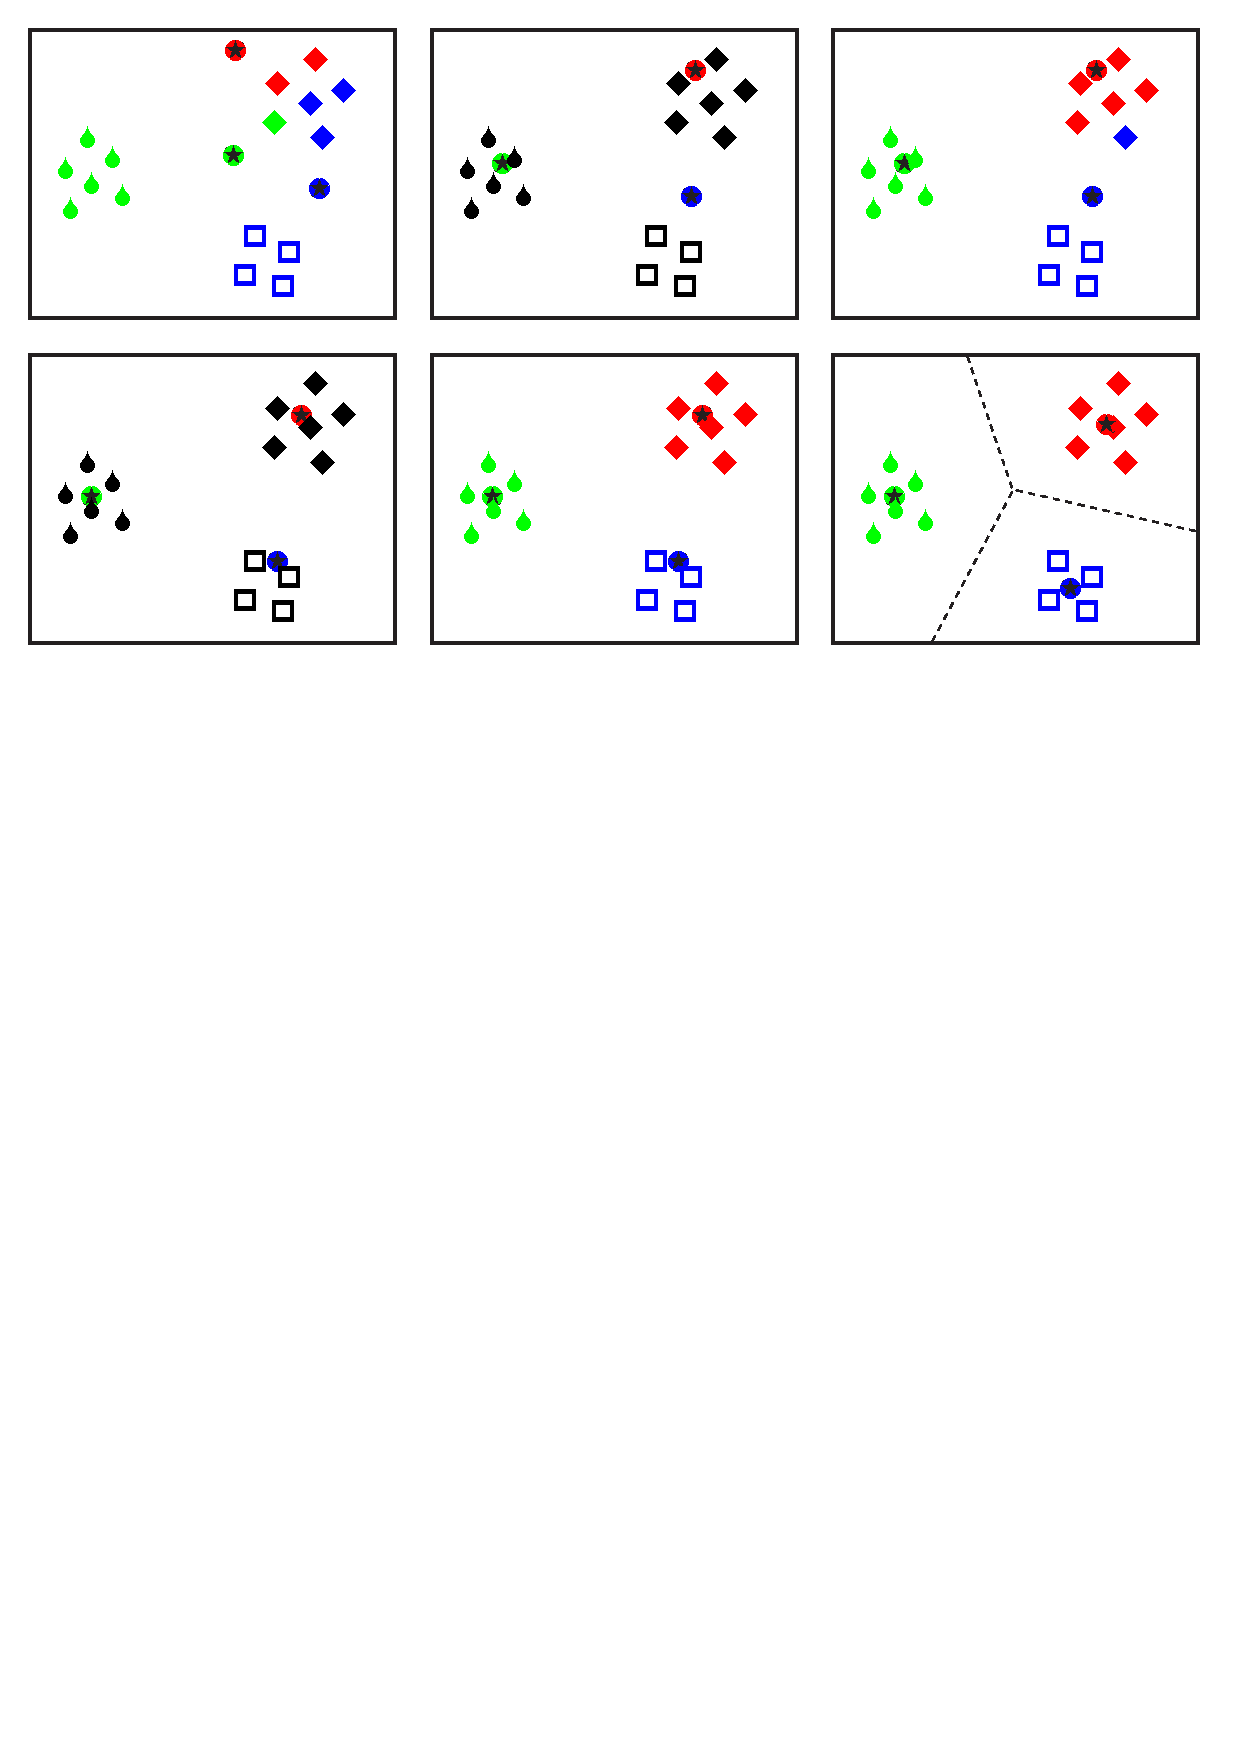
\includegraphics[width=.95\textwidth]{kmeans/lernenEinfach.pdf}
\caption{Trainingsphase beim k-Means Algorithmus}
\label{fig:lernenEinfach}
\end{figure*}

%\begin{figure}[htbp] \centering
%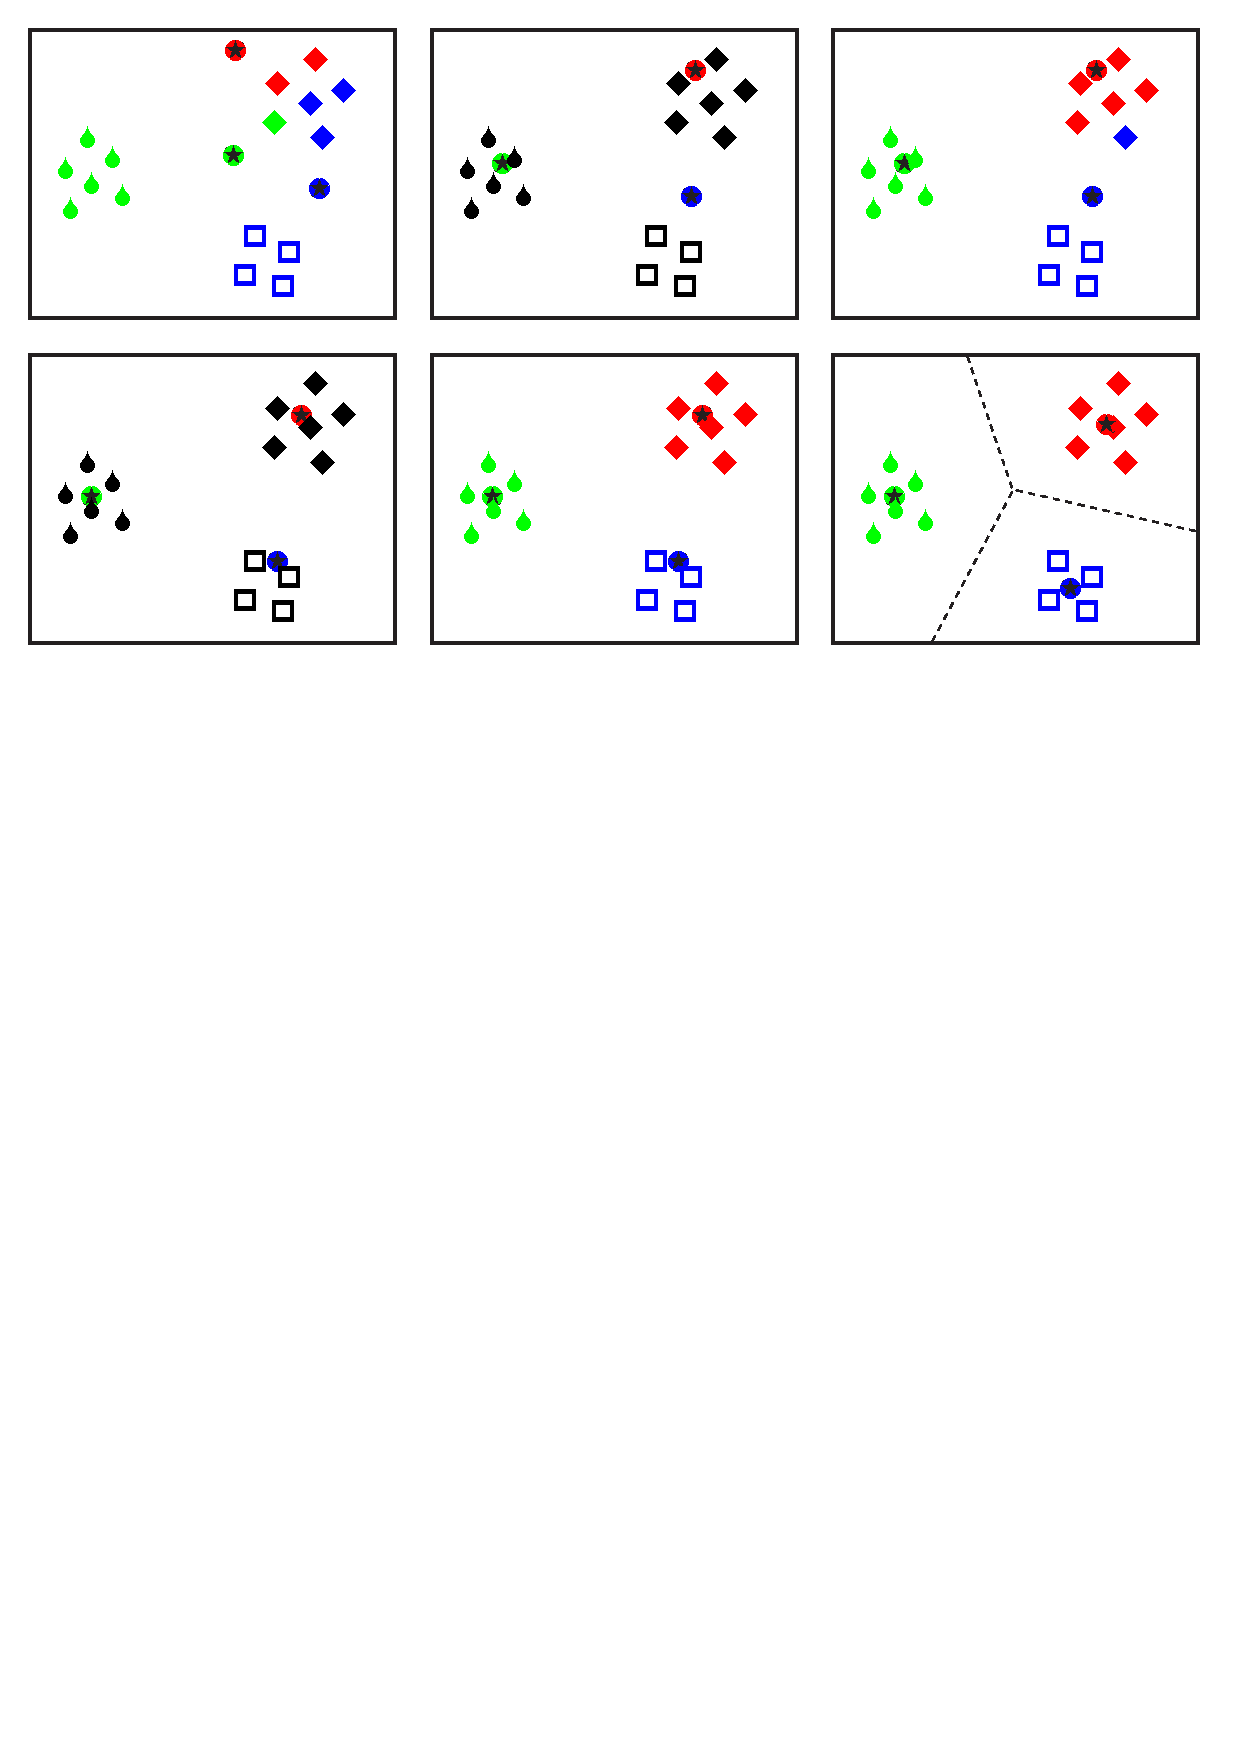
\includegraphics[height=60mm]{kmeans/lernenEinfach.pdf}
%\caption{Lernvorgang}
%\label{fig:lernenEinfach2}
%\end{figure}


Zu Beginn der Lernphase des Algorithmus wird ein Wert für \emph{k} festgelegt und anschließend werden \emph{k} zufällige Positionen im Eingaberaum als Cluster-Zentren gesetzt (siehe \autoref{fig:lernenEinfach}, oben links). Danach wird jedes Zentrum in den Schwerpunkt der ihm zugeordneten Objekte verschoben, sodass der Abstand zwischen Cluster-Zentrum und zugeordneten Objekten minimal wird. Diese Verschiebungen werden solange wiederholt, bis sich die Cluster-Zentren nicht mehr bewegen. 
Um nun zu einem Objekt das passende Cluster-Zentrum zuzuordnen, wird der Abstand zwischen Objekt und den Cluster-Zentrum berechnet. Das Objekt wird nun dem Cluster-Zentrum mit dem geringsten Abstand zugeordnet. In \autoref{fig:lernenEinfach} unten rechts ist  eine solche Bestimmung anhand der zuvor berechneten Cluster-Zentren dargestellt. Die Zugehörigkeit beliebiger Objekte zu den jeweiligen Cluster-Zentren ist durch Trennlinien markiert.
%, sodass ein zu klassifizierendes Objekt 
%dem Cluster das der Farbe entsprechende Cluster zugeordnet wird.


K-Means benötigt in der Regel beim Lernen mehr Zeit als bei der Benutzung, da im ersten Fall die Cluster-Zentren unter Umständen oft verschoben werden müssen und nach jeder Verschiebung erneut die Abstände zu allen dem Zentrum zugeordneten Punkten berechnet werden müssen. Bei der Benutzung hingegen genügt es, nur die Abstände des zu klassifizierenden Punkts zu allen Cluster-Zentren zu berechnen, um das passende Cluster zu bestimmen. Der Algorithmus arbeitet jedoch
% im Vergleich zu anderen Klassifikatoren (Beispiel??) in beiden Phasen schnell,
in beiden Phasen verhältnismäßig schnell, da immer nur 
der -- rechnerisch wenig aufwändige -- euklidische Abstand ermittelt wird.
Weiterhin ist festzuhalten, dass k-Means anfällig für Ausreißer ist, d.h. einzelne falsche Daten wie beispielsweise Messfehler können ein Cluster-Zentrum unter Umständen stark verschieben.
% einfache Berechnungen des euklidischen Abstands im Eingaberaum erfolgen.

Es existieren weiterhin einige Variationen des Basis-Algorithmus, mit dem dieser weiter optimiert werden kann. Dazu gehört etwa ein vorzeitiger Abbruch des Lernens, wenn eine festgelegte Maximalzahl von Iterationen erreicht wurde. Mit dem k-Means++ Algorithmus \cite{kMeans++} kann die Dauer der Lernphase verkürzt und die Fehlerrate bei der Benutzung gesenkt werden. Dieser Algorithmus wird in der Initialisierungsphase zur Bestimmung der Startpositionen der Cluster-Zentren verwendet. Dabei werden die Startpositionen der Cluster-Zentren nicht wie beim ursprünglichen Algorithmus zufällig gewählt, sondern wie folgt aus allen Eingabedaten $X$ bestimmt:
\begin{itemize}
\item Als erstes Cluster-Zentrum wird zufällig gleichverteilt ein Punkt aus $X$ gewählt.
\item Ein weiteres Cluster-Zentrum wird folgendermaßen ermittelt: 
\begin{itemize}
\item Die Entfernung $D(x)$ von allen Datenpunkten $x$ zu dem Cluster-Zentrum mit dem jeweils geringsten Abstand wird berechnet. 
\item Als neues Cluster-Zentrum wird zufällig ein Punkt aus den Eingabedaten bestimmt, wobei jeder Punkt $x$ mit der Wahrscheinlichkeit $\frac{ D(x)^{2} }{\sum\nolimits_{x \in X}D(x)^{2}}$ gewählt wird.
\end{itemize}
\item Der vorherige Schritt wird solange wiederholt, bis die gewünschte Menge an Cluster-Zentren berechnet ist.
\item Anschließend wird mit der Trainingsphase des ursprünglichen k-Means Algorithmus fortgefahren.
\end{itemize}


\subsection{Anwendung auf Projekt}
%oder andere Bewegungen beim Bedienen des Rechners 
Selbstverständlich wird versucht, die Fehlerquote bei der Gestenerkennung zu minimieren. Dabei ist es jedoch besonders wichtig, dass das Grundrauschen nicht fälschlicherweise als Geste erkannt wird. In einem solchen Fall würde es zu einer ungewollten Steuerung ohne Bewegung des Benutzers kommen, da die Aktion der irrtümlich erkannten Geste ausgeführt wird. Ebenso sollten andere Bewegungen beim Bedienen des Rechners wie etwa das Tippen auf der Tastatur oder eine Bewegung der Maus möglichst nicht als Geste erkannt werden.
Weniger bedeutend ist es hingegen, wenn umgekehrt eine Geste als Grundrauschen klassifiziert wird. In diesem Fall wird der Anwender die Geste wiederholen, bis diese erkannt und die zugeordnete Aktion ausgeführt wird.

Zur besseren Erkennung der Gesten ist es notwendig, die Rohdaten vor der Klassifikation zu filtern. Diese Vorverarbeitung wird in \autoref{subsubsec:Datenaufbereitung} näher beschrieben.

Zur Erkennung des Grundrauschens gibt es zwei Möglichkeiten: Entweder können eine oder mehrere weitere Klassen eingeführt werden, die für das Grundrauschen stehen. Oder der maximale Abstand von Geste und Cluster-Zentrum wird auf einen Maximalwert begrenzt, sodass
eine Aufnahme als Grundrauschen klassifiziert wird, wenn der Abstand zu allen Cluster-Zentren den Maximalwert überschreitet.
In ersten Tests zeigte sich, dass eine Erkennung des Grundrauschens mit einer zusätzlichen Klasse zuverlässig funktioniert. Daher wurde die zweite Variante eines maximalen Abstands zu den Cluster-Zentren -- die zusätzlichen Aufwand für die Anpassung der verwendeten Bibliothek sowie zur Ermittlung dieses Maximalwerts verursacht hätte -- nicht weiter verfolgt.


\subsubsection{Datenaufbereitung}\label{subsubsec:Datenaufbereitung}
% beim Überschreiten dieses Wertes die Aufnahme nicht als Geste, sondern als Grundrauschen klassifiziert wird.
%Zur Erkennung des Grundrauschens gibt es zwei Möglichkeiten: Entweder eine oder mehrere „Bullshit-Klassen“ einführen, die Aufnahmen entsprechen, bei denen keine (bekannte) Geste ausgeführt wurde. Die zweite Möglichkeit ist, den maximalen Abstand einer Geste zum nächstgelegenen Cluster-Center zu begrenzen, sodass beim Überschreiten des Grenzwerts „keine Geste“ klassifiziert wird.

%2 Cluster für Hintergrundrauschen, eins für leise und eins für laute Umgebung
%Ziel: Besser eine Geste fälschlicherweise als Grundrauschen einstufen und nicht erkennen, als das Grundrauschen oder andere Bewegungen beim Bedienen des Rechners als Geste einstufen. Im ersten Fall wird der Anwender die Geste einfach erneut ausführen (und sie wird dann – hoffentlich – auch erkannt), im zweiten Fall ist es nervig, da die mit der erkannten Geste verknüpfte Aktion ausgeführt wird. 

Die Rohdaten einer Aufnahme bestehen aus 32 Frames, die jeweils 64 Lautstärkewerte beinhalten. Jeder Lautstärkewert entspricht dabei der Intensität des Tonsignals in dem jeweiligen Frequenzbereich, welche mithilfe der schnellen Fourier-Transformation (\emph{FFT}) \cite{fftMathebuch} berechnet wurde. Jede einzelne Aufnahme besteht daher aus $32 \cdot 64 = 2048$ Dimensionen.  Da hochdimensionale Eingabedaten bei Clustering-Verfahren oft schlechte Ergebnisse liefern \cite{kMeansHighDimensions}, ist es notwendig, bei der Datenaufbereitung die Dimension der Eingabedaten zu reduzieren.  Erste Tests mit nicht aufbereiteten 2048-dimensionalen Eingabedaten lieferten eine korrekte Erkennungsrate von etwa 25 bis 30 Prozent bei 6 Klassen (5 Gesten sowie Grundrauschen ohne Geste). Lediglich das Grundrauschen kann so einigermaßen zuverlässig erkannt werden, eine korrekte Unterscheidung der einzelnen Gesten ist jedoch nicht möglich. Dies zeigt deutlich die Notwendigkeit einer Datenaufbereitung.

%TODO
TODO: Datenaufbereitung beschreiben 

%2048 Dimensionen. 
%Die Rohdaten einer Aufnahme haben die Größe von $32 Frames \cdot 64 Lautstärkewerte  = 2048 Dimensionen$.
%Rohdaten sind zu hochdimensional, um ohne Vorverarbeitung in den Klassifikator gesteckt werden zu können. Bei der verwendeten Implementierung (siehe später) sind pro Geste beispielsweise 32 Frames $\cdot$ 64 Lautstärkewerte, die je einem Frequenzbereich entsprechen (siehe FFT \cite{fftMathebuch}), = 2048 Daten vorhanden.
% Da hochdimensionale Eingabedaten bei Clustering-Verfahren oft schlechte Ergebnisse liefern \cite{kMeansHighDimensions}, ist es notwendig, bei der Datenaufbereitung die Dimension der Eingabedaten zu reduzieren. 


\subsubsection{Anpassung des Klassifikators}
Der Klassifikator wurde nur geringfügig angepasst.
In der Initialisierungsphase werden die Startpunkte der Cluster-Zentren wurden nicht wie im ursprünglichen Algorithmus zufällig gewählt, sondern mithilfe des in \autoref{subsec:kMeansFunktionsweise} vorgestellten k-Means++ Algorithmus bestimmt. Die Trainingsphase läuft hingegen unverändert ab.
% Die Startpunkte der Cluster-Zentren wurden nicht wie im ursprünglichen Algorithmus zufällig gewählt, sondern mithilfe des in \autoref{subsec:kMeansFunktionsweise} vorgestellten k-Means++ Algorithmus bestimmt.
 Dadurch ergeben sich in der Regel eine schnellere Laufzeit in der Trainingsphase sowie bessere Ergebnisse bei der Klassifikation.
% Klassifikationsergebnisse. 
Ansonsten wurden keine Veränderungen am Algorithmus vorgenommen.
%keine, kMeans++ für Optimierung von Geschwindigkeit und Erkennungsrate, hohe Anzahl für maxIter, da Algorithmus schnell ist, precomputeDistances=True, da Kl

Für die Qualität der Klassifikation ist weiterhin jedoch die Wahl eines geeigneten Werts für \emph{k} von Bedeutung. Dabei muss \emph{k} mindestens um eins größer sein als die Anzahl der Gesten (da mindestens eine Klasse für das Grundrauschen benötigt wird),
%gleich der Anzahl der Gesten +  sein
damit der Algorithmus in der Lage ist, die einzelnen Aufnahmen voneinander zu unterscheiden.  

%Die größte "Anpassung" ist die Wahl eines geeigneten Werts für k. Ausprobieren, ob k=Anzahl Gesten (+Grundrauschen) bereits gute Ergebnisse liefert, ansonsten größere Werte für k wählen und manchen Gesten mehr als ein Cluster-Zentrum zuordnen.
% Es existieren zwar Faustregeln/Algorithmen, wie k gewählt werden kann, aber die sind hier weniger geeignet
%ansonsten keine Anpassungen vorgenommen.( da es sich um einen einfachen Algorithmus handelt, der wenig Möglichkeiten zur  Anpassung bietet
%Die Anzahl der zu bestimmenden Cluster -- d.h. der Wert von \emph{k} -- muss bereits vor der Trainingsphase festgelegt werden. Dabei muss \emph{k} mindestens gleich der Anzahl der Gesten sein, damit der Algorithmus in der Lage ist, die einzelnen Gesten voneinander zu unterscheiden. 

Grundsätzlich gibt es zur Ermittlung der Anzahl an Clustern in einem Datensatz viele verschiedene Ansätze, etwa die Faustregel $k \approx \sqrt{n/2}$ \cite{WikipediaKMeansKValue}, wobei \emph{n} der Anzahl der Datenpunkte entspricht. In Fall der hier beschriebenen Gestenerkennung kann der Wert für \emph{k} jedoch bereits grob abgeschätzt werden. 
%Die untere Grenze ist wie bereits erwähnt gleich der Anzahl der Gesten + 1.
Die untere Grenze ist wie bereits erwähnt um eins größer als die Anzahl der Gesten.
Als obere Grenze lässt sich grob der fünffache Wert der unteren Grenze abschätzen, da davon auszugehen ist, dass es nur wenige Variationsmöglichkeiten beim Ausführen einer Geste gibt.
%Denkbar sind hierbei beispielsweise zwei solcher zusätzlicher Gruppen, eine für das Hintergrundrauschen ohne Bewegung und eine weitere für alle Bewegungen, die keiner gespeicherten Geste entsprechen.







%TODO Zuordnung Cluster-Zentren zu Gesten ausformulieren
Nach der Lernphase ist es noch notwendig, dass den einzelnen Cluster-Zentren je eine Geste zugeordnet wird. Dazu wird ermittelt, welche Geste wie oft in die einzelnen Cluster-Zentren eingeordnet wird. Falls \emph{k} gleich dem oben genannten Minimalwert ist, ist es ausreichend, dem ersten Cluster die am häufigsten dort vorkommende Geste zuzuordnen, dem zweiten Cluster die häufigste vorkommende Geste der übrigen Gesten etc. 
Somit ergibt sich 
%folgender Algorithmus
Algorithmus 1 
zur Zuordnung je einer Geste zu dem jeweiligen Cluster-Zentrum, in welches sie am meisten fällt.
\begin{itemize}
    
    \item für alle Gesten:
    \begin{itemize}
    
        \item suche in der Liste der Cluster das Cluster, in das die Geste am häufigsten fällt
        \item speichere Zuordnung Cluster->Geste
        \item entferne gefundenes Cluster aus der Liste
        \end{itemize}

    \item (Ergebnis: Zuordnung Cluster->Geste mit AnzahlGesten Einträgen)

\end{itemize}

%TODO ggf siehe Listing XX
Ist \emph{k} größer als der Minimalwert, werden zuerst die \emph{k} Cluster, bei denen die Anzahl der am häufigsten zugeordneten Geste maximal ist, gemäß 
%dem vorherigen Algorithmus
Algorithmus 1
durchlaufen und jedem dieser Cluster eine andere Geste zugeordnet. Anschließend wird jedem übrigen Cluster die Geste zugeordnet, die am häufigsten in das Cluster eingeordnet wurde.
Insgesamt ergibt sich also folgender Ablauf:
    ALGO 2: Übrige Cluster Gesten zuordnen
    \begin{itemize}
	\item Erstelle Zuordnung Cluster->Geste gemäß Algorithmus 1
    \item erstelle Cluster-Liste, die alle noch nicht zugeordneten Cluster enthält
    \item für alle Cluster:
    \begin{itemize}

        \item suche in der Liste der Gesten die Geste, die am häufigsten in das Cluster fällt
        \item speichere Zuordnung Cluster->Geste
        \item (entfernen des Clusters nicht nötig und i.d.R. auch nicht möglich)
        \end{itemize}
   \end{itemize}

%TODO Was ist der " vorherigen Algorithmus"??
%TODO Was ist "dieser Algorithmus"??
%Dieser Algorithmus arbeitet 
Beide Algorithmen arbeiten
zuverlässig, wenn die Gesten -- bis auf wenige Ausnahmen -- eindeutig einem Cluster zugeordnet werden können. Ist dies nicht der Fall, kann keine akzeptable Gestenerkennung realisiert werden und die Vorverarbeitung und/oder der Wert von \emph{k} sollte angepasst werden.
% Falls \emph{k} gleich dem 

%Wahl von optimalen Wert für k, in diesem Anwendungsfall (natürlich) mindestens Anzahl der Gesten, aber auch größere Werte möglich. Im einfachen Fall \emph{k} = AnzahlGesten wird jedem Clustercenter eine Geste zugeordnet. Im Idealfall wenig Überlappung der Confusion Matrix, sodass bei jeder Geste ein eindeutiges Cluster am häufigsten vorkommt und umgekehrt in jedes Cluster eine einzige Geste am häufigsten fällt (Später bei\emph{ k } $>$ AnzahlGesten muss das nicht für jedes Cluster gelten, aber mindestens für\emph{ k }Stück). Wenn\emph{ k }größer ist als die Anzahl der Gesten, sind mindestens einer Geste mehrere Cluster-Schwerpunkte zugeordnet. $->$ Algorithmus, um Clustercenter den einzelnen Gesten zuzuordnen. 


%Wahl eines guten Werts für\emph{ k }von Bedeutung, offensichtlich mindestens Anzahl der Gruppen (wenn Anzahl der Gruppen vorher bekannt ist). Verschiedene Methoden, die einfachste ist die Faustregel, dass  (REF).
%Quelle:  Faustregel: Kanti Mardia et al. (1979). Multivariate Analysis. Academic Press. (via http://en.wikipedia.org/wiki/Determining_the_number_of_clusters_in_a_data_set)



%Bei dem k-Means Algorithmus ist zu beachten, dass die Anzahl der Cluster vorher bekannt sein muss, da sie beim Start des Algorithmus festgelegt wird. Dies ist jedoch kein Problem, weil die Anzahl der Gesten im Erkennungssystem auf eine bestimmte Zahl (voraussichtlich 6) festgelegt ist. Da der Klassifikator jede beliebige Eingabe einem der Cluster zuordnet, ist es notwendig, eine oder mehrere zusätzliche Gruppen für nicht erkannte Gesten zu definieren. Ansonsten würde jede Eingabe – unabhängig ob es tatsächlich eine Geste war oder nicht – grundsätzlich der ähnlichsten bekannten Gesten zugeordnet. 
%Die Features zur Klassifikation müssen so gewählt werden, dass sich gleiche Gesten im gleichen Cluster anordnen und es möglichst nicht zu einer Überschneidung von verschiedenen Clustern kommt. Dies ist notwendig, da der Klassifikator ansonsten nicht mehr in der Lage ist, die einzelnen Gesten voneinander zu unterscheiden. Anhand des im aktuellen Prototyp dargestellten Frequenzspektrums lässt sich erkennen, dass sich die Gesten weniger durch die zu einem bestimmten Zeitpunkt gemessenen Frequenzwerte unterscheiden lassen, sondern eher durch den zeitlichen Verlauf dieser Frequenzwerte von Beginn bis Ende der Geste.



\subsubsection{Implementierung} \label{subsubsec:kMeansImpl}
Die Implementierung erfolgt in der Programmiersprache Python unter Verwendung der Bibliothek skikit-learn (Version 0.14) \cite{sklearn}. Diese Bibliothek verwendet den beschriebenen k-Means Algorithmus von Lloyd. Außerdem bietet sie noch die Möglichkeit, dass die Startpunkte der Cluster-Zentren nicht wie im ursprünglichen Algorithmus vorgesehen zufällig gewählt werden, sondern stattdessen mit dem k-Means++ Algorithmus \cite{kMeans++} bestimmt werden. Zusätzlich können noch weitere 
%kleine 
Einstellungen vorgenommen werden, um den Klassifikator für den jeweiligen Anwendungsfall  zu optimieren. Dazu gehört beispielsweise eine Beschränkung der Iterationen beim Lernen auf einen bestimmten Maximalwert.
Die Komplexität im ungünstigsten Fall liegt bei $O(n^{(k+2)/p})$ \cite{sklearn.kmeans, kMeansHowSlow}, wobei $n$ der Anzahl der Trainingsdaten und $p$ der Anzahl der Dimensionen entspricht.


\subsubsection{Evaluation}
TODO: Confusion Matrix in lauter und leiser Umgebung für die verschiedenen Gesten. Welche Gesten werden sehr gut/gut/mittelmäßig oder gar nicht erkannt? Ist die Erkennungsrate praxistauglich?

\subsection{Fazit}
Wie gut funktioniert die Erkennung? Welche Gesten werden gut, welche schlecht erkannt? Ausblick auf potentielle weiterführende Arbeiten.
%Die Erkennung funktioniert mittelmäßig/gut/sehr gut. Sehr gut erkannt werden das Grundrauschen und Geste(n) . Schlecht/kaum erkannt werden Geste(n)  (siehe Confusion Matrix). Ausblick auf potentielle weiterführende Arbeiten